% !TEX root = main.tex
\chapter[head={Der Zerfallskanal $\Bz\rightarrow \Dm\pip$ und dessen Selektion},tocentry={Der Zerfallskanal $\mathbf{\Bz\rightarrow \Dm\pip}$ und dessen Selektion}]{Der Zerfallskanal $\mathbf{\Bz\rightarrow \Dm\pip}$ und dessen Selektion}

Die im Folgenden verwendeten Daten stammen aus Proton-Proton Kollisionen am \lhc aus den Jahren 2011 und 2012, korrespondierend zu Schwerpunktsenergien von $\sqs=\SI{7}{TeV}$ und $\sqs=\SI{8}{TeV}$. Dies entspricht integrierten Luminositäten von \SI{1{,}0}{fb^{-1}} für das Jahr 2011 und \SI{2{,}0}{fb^{-1}} für das Jahr 2012.\\
Im Folgenden ist mit $\Bz\rightarrow \Dm\pip$ implizit auch immer der ladungskonjugierte Zerfall $\Bzb\rightarrow \Dp\pim$ eingeschlossen. In diesem Kapitel wird nun auf die experimentellen Vorarbeiten für die Kalibrierung des Flavour Taggings im Kanal $\Bz\rightarrow \Dm\pip$ eingegangen werden. Dazu wird zunächst der Zerfall selbst näher beleuchtet, um danach auf die vorgenommene Selektion und das verwendete Fitmodell einzugehen.

\section[head={Rekonstruktion des Kanals $\Bz\rightarrow \Dm(\rightarrow \Kp\pim\pim)\pip$},tocentry={Rekonstruktion des Kanals $\Bz\rightarrow \Dm(\rightarrow \Kp\pim\pim)\pip$}]{Rekonstruktion des Kanals $\mathbf{\Bz\rightarrow \Dm(\rightarrow \Kp\pim\pim)\pip}$}

Bei dem Zerfallskanal $\Bz\rightarrow\Dm(\rightarrow \Kp\pim\pim)\pip$ handelt es sich um einen selbsttaggenden Kanal mit rein hadronischem Endzustand. Selbsttaggend bedeutet dabei, dass aus den Zerfallsprodukten auf den Flavour des \B-Mesons zum Zeitpunkt des Zerfalls geschlossen werden kann. Weiterhin handelt es sich um einen Endzustand, der sich nur aus geladenen Teilchen zusammensetzt, wodurch alle Teilchen im Detektor gut nachzuweisen sind. Da es sich jedoch, um einen rein hadronischen Endzustand handelt, ist bei der Selektion (Kapitel \ref{sec:selektion}) und Analyse auf nicht flache Untergründe, bedingt durch Fehlrekonstruktionen oder -identifikationen, zu achten. Diese sind hier wahrscheinlicher, da Pionen und Kaonen im Experiment deutlich schwerer zu unterscheiden und identifizieren sind, als beispielsweise Myonen.\\
Es handelt sich bei $\Bz\rightarrow \Dm\pip$ jedoch nicht um einen vollständig selbsttaggenden Zerfall, da auch der Zerfall $\Bz\rightarrow D^+\pim$ (Abbildung \ref{fig:b2dpi}) möglich ist. 
\begin{figure}[htpb]
	\centering
		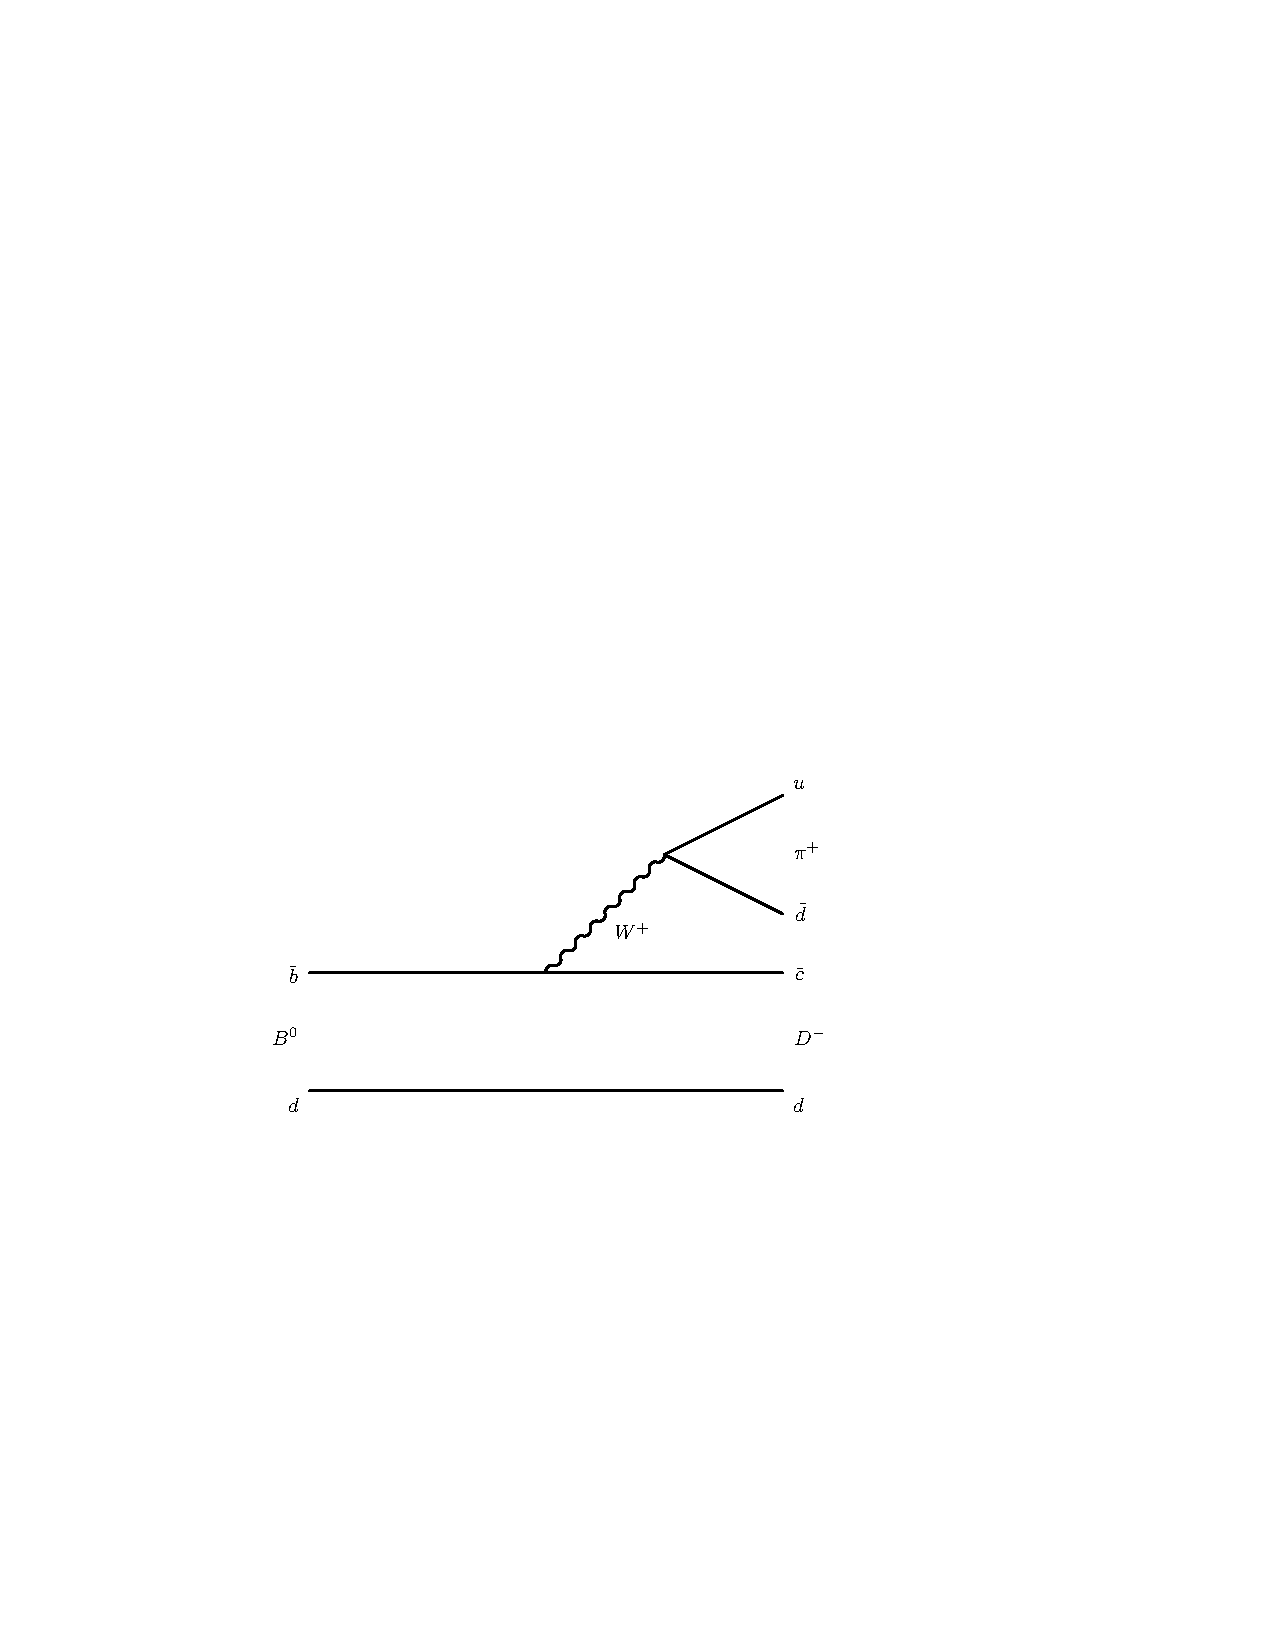
\includegraphics[width=0.45\textwidth]{fig/B2D-pi+.pdf}
		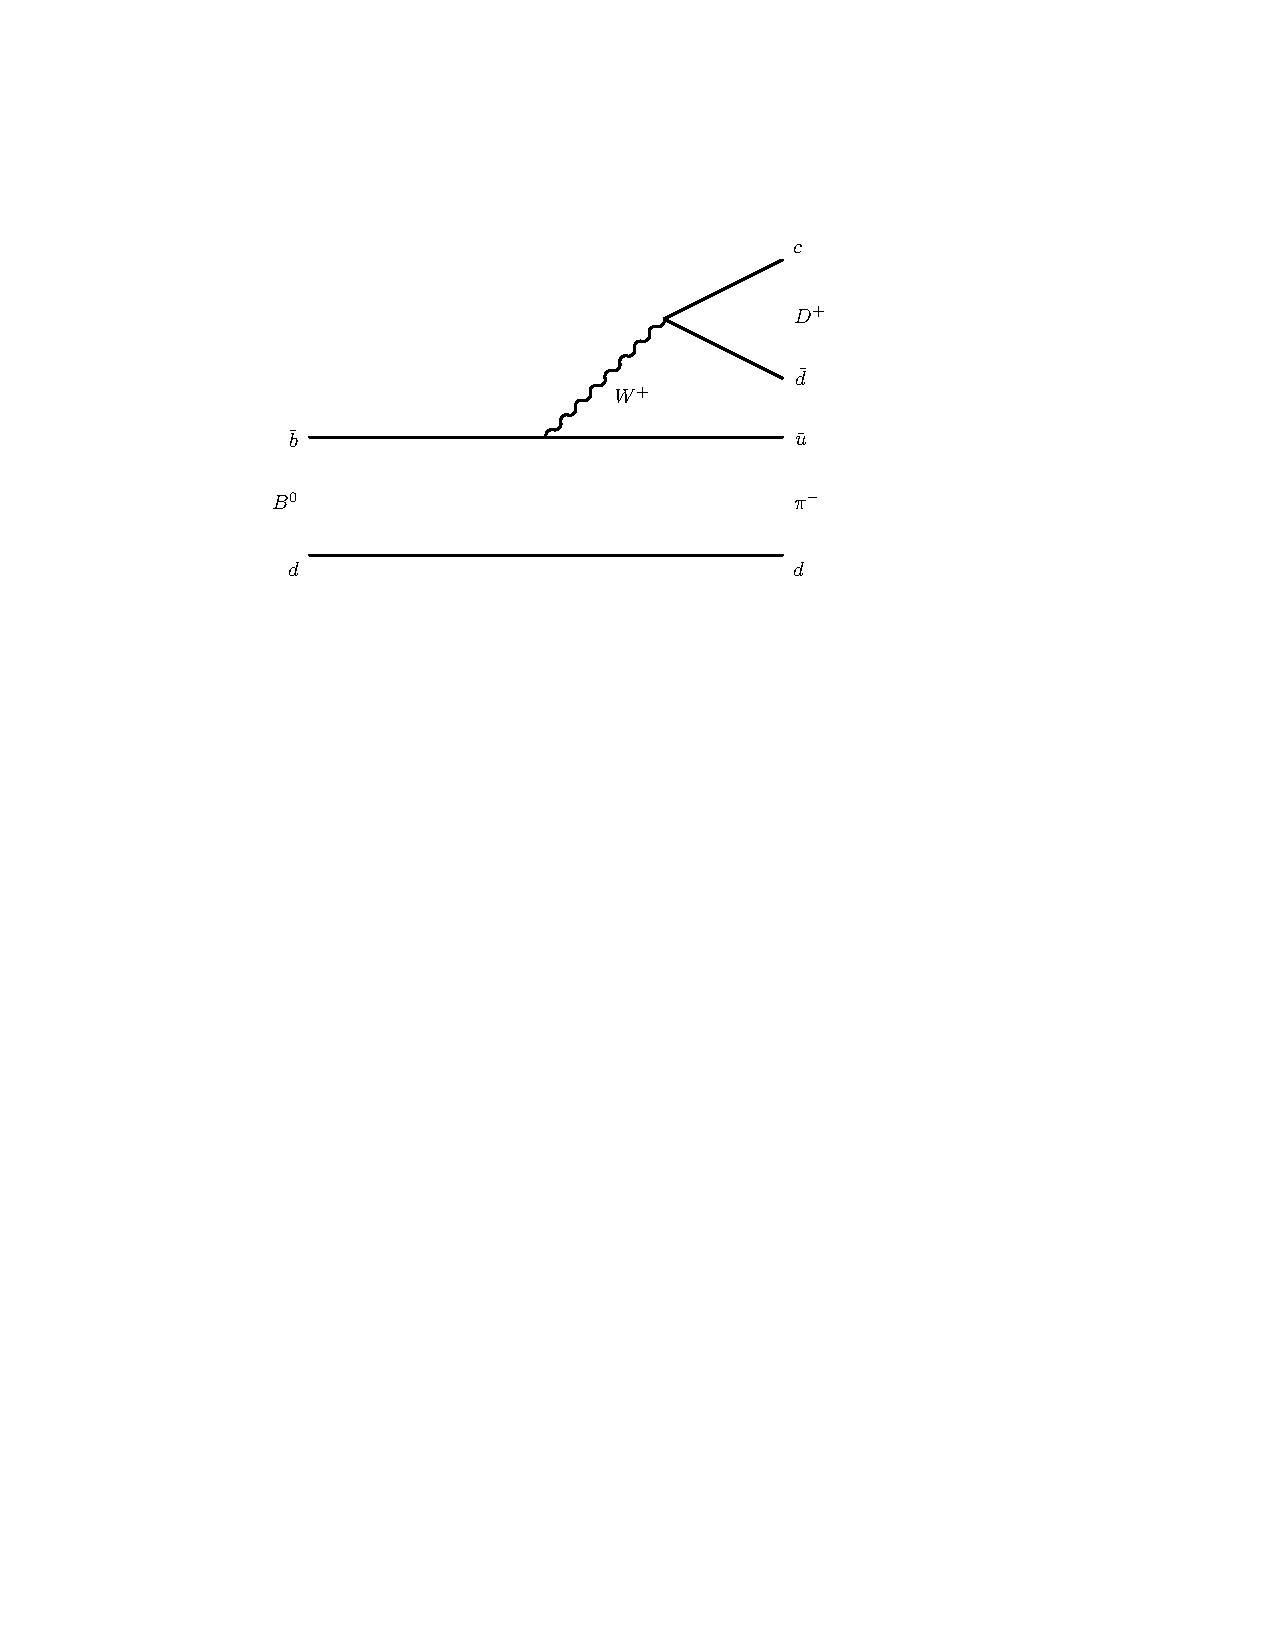
\includegraphics[width=0.45\textwidth]{fig/B2D+pi-.pdf}
	\caption{Feynmandiagramme niedrigster Ordnung der beiden Zerfälle des neutralen \B-Mesons in geladene $D\pi$ Endzustände. Rechts der Zerfall $\Bz\rightarrow D^+\pim$, der gegenüber dem in dieser Arbeit betrachtete Zerfall $\Bz\rightarrow \Dm\pip$ $C\!K\!M$ unterdrückt ist.}
	\label{fig:b2dpi} 
\end{figure}  
Im Kanal $\Bz\rightarrow \Dm\pip$ ist die Zerfallsamplitude proportional zu $\Vud\Vcb\propto\lambda^2$, im Kanal $\Bz\rightarrow D^+\pim$ jedoch nur zu $\Vub\Vcd\propto\lambda^4$ (siehe Gleichung \eqref{eq:wolfen}), sodass dieser zweite Kanal $C\!K\!M$ unterdrückt ist. Aus diesem Grund lässt sich $\Bz\rightarrow \Dm\pip$ trotzdem zur Kalibrierung des Flavour Taggings nutzen. Allerdings muss beachtet werden, dass Einflüsse des $C\!K\!M$ unterdrückten Zerfalls einen Einfluss auf die Messung der true-mistag-Wahrscheinlichkeit $\omega$ haben kann. \\
Der Zerfall $\Bz\rightarrow \Dm\pip$ wird im Folgenden aus dem weiteren Zerfall $\mbox{\Dm\rightarrow \Kp\pim\pim}$ und einem geladenen Tochter Pion rekonstruiert.

\section{Selektion}\label{sec:selektion}

Für die Rekonstruktion von Ereignissen mit dem Zerfall $\Bz\rightarrow \Dm\pip$ werden vier HLT Trigger verwendet, drei sogenannte Topo Trigger und eine inklusiver $\phi$ Trigger. Die Topo Trigger fordern gut rekonstruierte Kandidaten mit einem Sekundärvertex aus zwei, drei oder vier Spuren. Für die inklusiven $\phi$ Trigger muss ein geladenes Kaon im Endzustand sein, da dass $\phi$  in etwa \SI{50}{\%} aller Fälle in zwei geladene Kaonen zerfällt. 
\begin{table}[tbp]
  \centering
     \caption{Schnitte der Vorselektion für den Kanal $\Bz\rightarrow \Dm\pip$ in der Stripping Version 20. Abweichende Schnitte für die Version 20r1 sind in Klammern gegeben. Die Größe $\chi^2$ ist dabei ein Maß für die Güte eines durchgeführten Fits.}
    \label{tab:stripping}
    \begin{tabular}{cc}
    \toprule
    \multicolumn{2}{c}{Schnitte auf \Bz-Kandidaten} \\
    \midrule
    Summe der Transversalimpulse \pt aller Teilchen & $>\SI{5000}{MeV\per \it{c}}$\\
    $\chi^2$ des Primär Vertex & $<25$ \\
    $\chi^2/\text{ndof}$ des Primär Vertex  & $<10$\\
    cos von $\sphericalangle\left[\left|PV,\Bz\text{Vtx}\right|, \vec{p}\left(\Bz\right)\right]$ & $<0{,}999$ \\
    Zerfallszeit & $>\SI{0{,}2}{ps}$\\
    $m\left(\kaon\pion\pion\pion\right)_\text{min}$ & \SI{4750}{MeV\per \it{c}^2}\\
    $m\left(\kaon\pion\pion\pion\right)_\text{max}$ & \SI{6000}{MeV\per \it{c}^2}\\ 
    \midrule
    \multicolumn{2}{c}{Schnitte auf \Dm-Kandidaten}\\ 
    \midrule
    Summe der Transversalimpulse \pt aller Teilchen & $>\SI{1800}{MeV\per \it{c}}$\\
    Vertex $\chi^2/\text{ndof}$ & $<10$\\
    bestes $\chi^2$ des Primär Vertex & $>36$\\
    cos von $\sphericalangle\left[\left|PV,\Dm\text{Vtx}\right|, \vec{p}\left(\Dm\right)\right]$ & $>0$ \\
    Maximaler Abstand der kleinsten Annäherung zum PV & $<\SI{0{,}5}{mm}$\\ 
    \midrule
    \multicolumn{2}{c}{Schnitte auf \Kp- und \pipm-Kandidaten}\\ 
    \midrule
    Transversalimpuls \pt & $>\SI{100}{MeV\per \it{c}}$\\
    Impuls $p$ & $>\SI{1000}{MeV\per \it{c}}$\\
    $\chi^2/\text{ndof}$ der Spur & $<3$\\
    ghost-Wahrscheinlichkeit der Spur & $<0{,}3$ ($<0{,}4$) \\
    kleinstes Stoßparameter $\chi^2$ & $>4$\\ 
    \bottomrule
    \end{tabular}
\end{table}
Obwohl der Zerfall $\Bz\rightarrow \Dm\pip$ kein $\phi$ enthält, ist dieser Trigger aufgrund des geladenen Kaons im Zerfall des \D-Mesons $\Dm\rightarrow \Kp\pim\pim$ geeignet.\\
Bei der weiteren Vorselektion, dem sogenannten Stripping, werden die Schnitte aus Tabelle \ref{tab:stripping} angewendet. Dabei wird zwischen den Jahren 2011 und 2012 mit den Stripping Versionen 20r1 und 20 unterschieden. Die finale Selektion wurde in Anlehnung an eine Analyse zur Messung der \Bs-Lebenszeit relativ zur \Bz-Lebenszeit durchgeführt \cite{selektion}. Sie unterteilt sich in rechtwinklige Schnitte und speziellere Massenvetos, um bestimmte nicht flache (peakende) Untergründe auszuschließen. Außerdem wurde in jedem Ereignis nur der Zerfall mit dem PV mit dem kleinsten $\chi^2$ des Stoßparameters gewählt. Die rechtwinkligen Schnitte sind in Tabelle \ref{tab:selektion} zu sehen.
\begin{table}[tbp]
  \centering
     \caption{Rechtwinklige Schnitte der finalen Selektion. Die Größe $\chi^2$ ist dabei ein Maß für die Güte eines durhcgeführten Fits, \dllkpi beschreibt die Wahrscheinlichkeit, ob es sich bei einem Teilchen eher um ein Kaon oder ein Pion handelt und \enquote{ist Myon} dient der Unterscheidung von Myonen.}
    \label{tab:selektion}
    \begin{tabular}{cc}
    \toprule
    \multicolumn{2}{c}{Schnitte auf \Bz-Kandidaten} \\ 
    \midrule
    größtes $\chi^2$ des Stoßparameters zu dem assoziierten PV & $<16$  \\ 
    cos von $\sphericalangle\left[\left|PV,\Bz\text{Vtx}\right|, \vec{p}\left(\Bz\right)\right]$ & $<0{,}9999$ \\
    Zerfallszeit & $>\SI{0{,}3}{ps}$\\ 
    $m\left(\kaon\pion\pion\pion\right)_\text{min}$ & \SI{5200}{MeV\per \it{c}^2}\\
    $m\left(\kaon\pion\pion\pion\right)_\text{max}$ & \SI{5500}{MeV\per \it{c}^2}\\ 
    \midrule   
    \multicolumn{2}{c}{Schnitte auf \Dm-Kandidaten} \\ 
    \midrule
    Zerfallszeit  & $>\SI{0}{fs}$  \\ 
    kleinstes $\chi^2$  der Flugdistanz mit dem SV & $>1$  \\ 
    kleinstes $\chi^2$ des Stoßparameters zu dem \Bz-PV & $>4$  \\ 
    $\left|m(\kaon\pion\pion)-m(\Dpm)_\text{PDG}\right|$ & $<\SI{25}{MeV \per \it{c}^2}$  \\
    \midrule
    \multicolumn{2}{c}{Schnitte auf \pip-Kandidaten} \\ 
    \midrule
    ist Myon & $=0$ \\ 
    kleinstes $\chi^2$ des Stoßparameters mit dem PV & $>36$  \\
    \dllkpi & $<2$  \\ 
    \midrule
    \multicolumn{2}{c}{Schnitte auf \Kp- und \pim-Kandidaten} \\ 
    \midrule
    kleinstes $\chi^2$ des Stoßparameters mit dem assoziierten PV & $>9$ \\
    \dllkpi für Pionen & $<5$  \\
    \dllkpi für \Kp & $>0$  \\ 
    \bottomrule
    \end{tabular}
\end{table}
Insgesamt erhält man nach allen rechtwinkligen Schnitten auf Monte-Carlo eine Signaleffizienz von \SI{73{,}24}{\%}. Bei den Massenvetos wurde auf zwei Untergründe eingegangen. Mit dem \Dsm-Veto soll der Zerfall $\Bs\rightarrow\Dsm\pip$ ausgeschlossen werden, das \Lc-Veto soll den Zerfall $\Lb\rightarrow\Lc\pim$ eliminieren:
\begin{figure}[tbp]
	\centering
		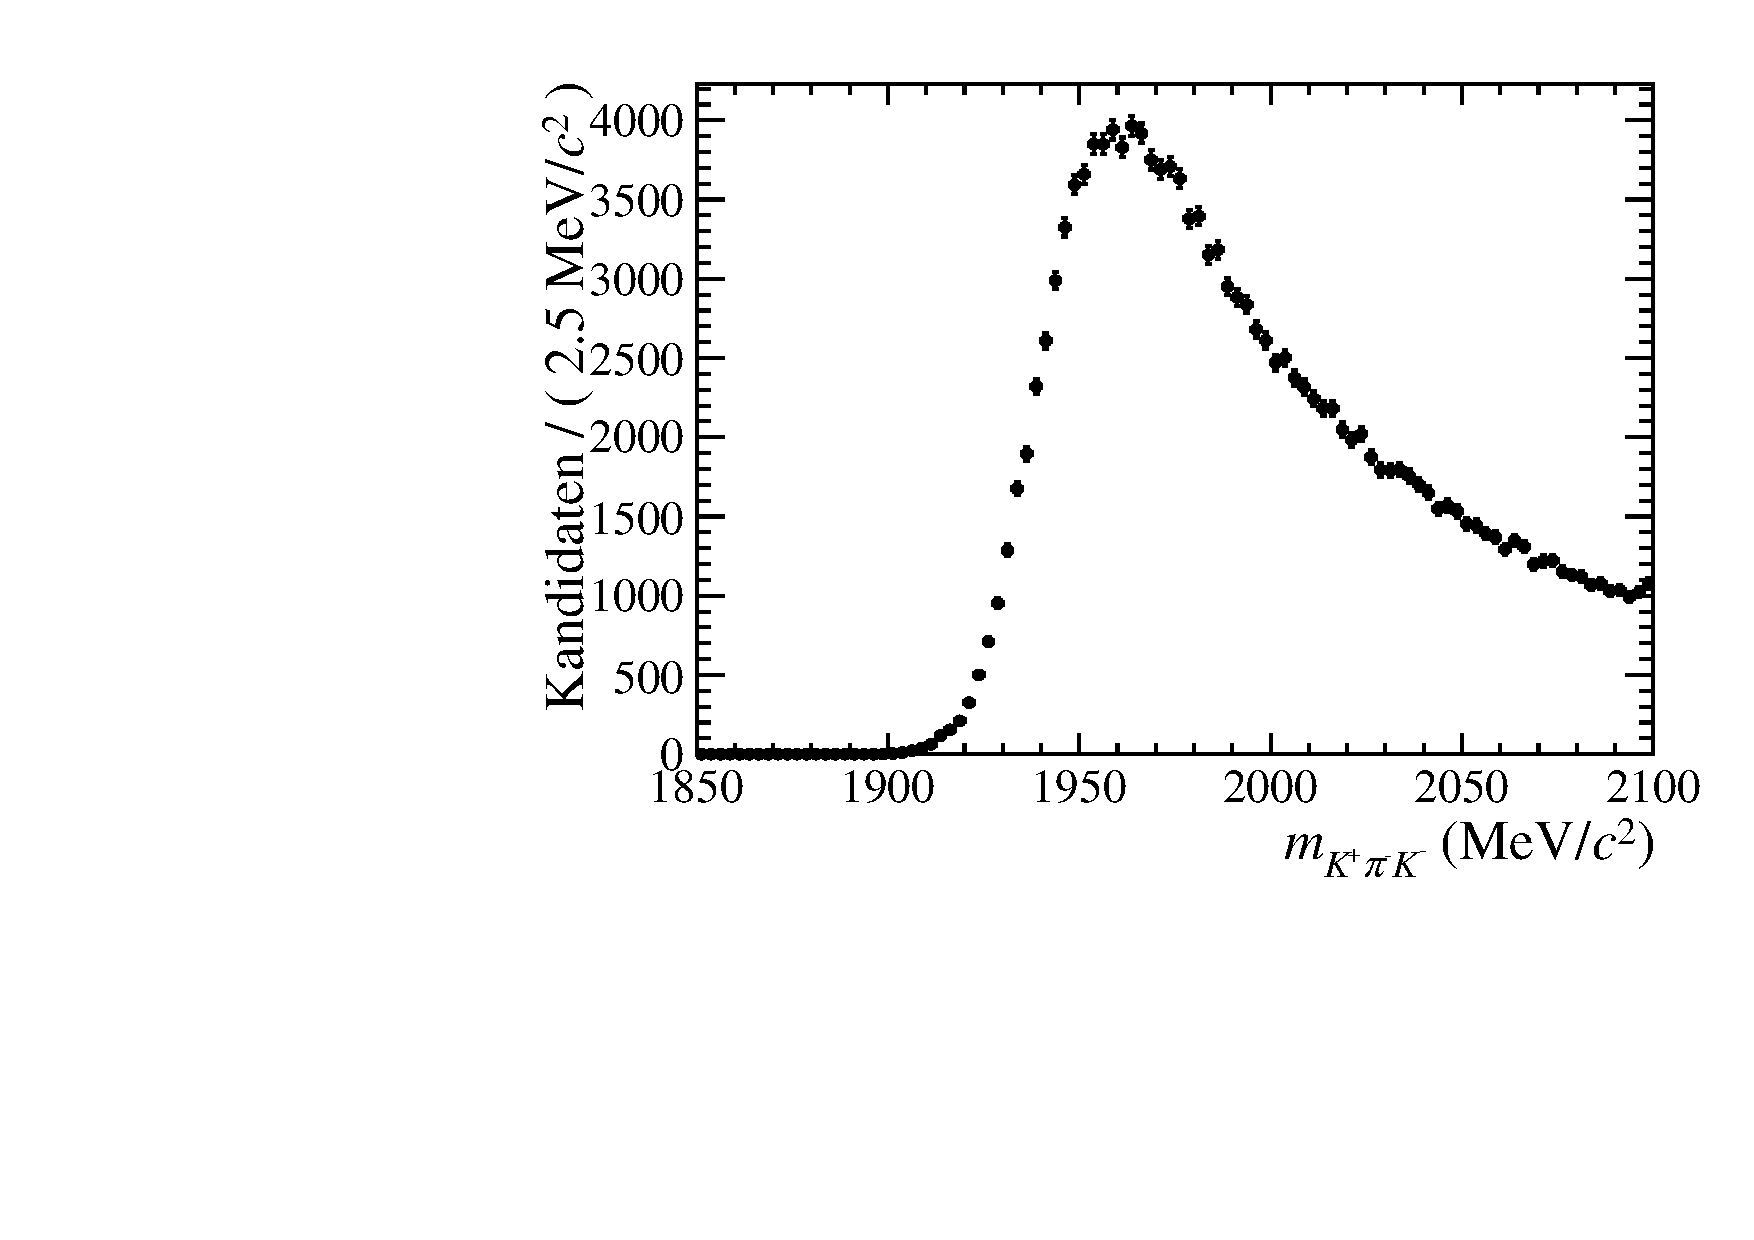
\includegraphics[width=0.45\textwidth]{fig/obsMass_Ds1.pdf}
		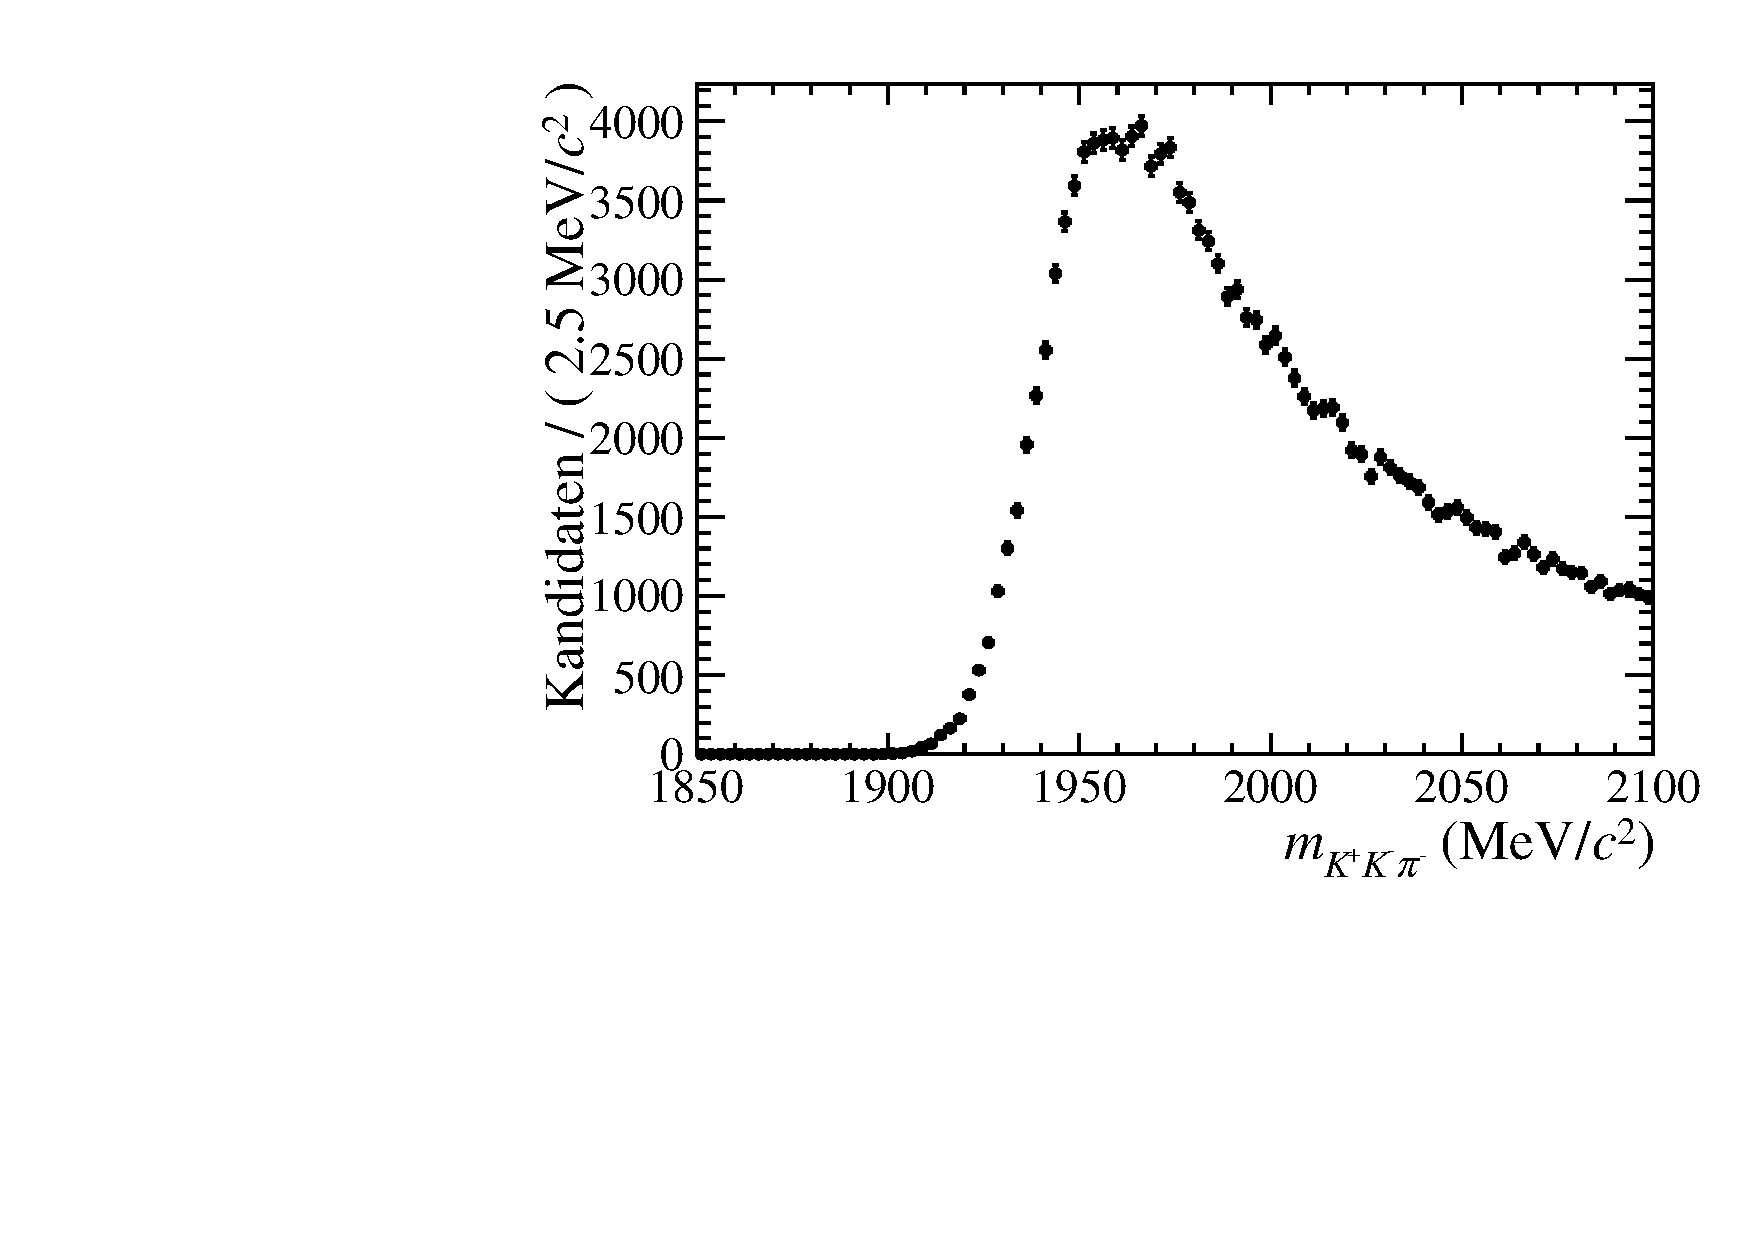
\includegraphics[width=0.45\textwidth]{fig/obsMass_Ds2.pdf}
	\caption{Massenverteilung der \Kp\pim\pim Kombination nach Anwendung einer Kaon Massenhypothese für ein \pim. Die Plots entsprechen den Massenverteilungen für die zwei möglichen Kombinationen.}
	\label{fig:dsveto} 
\end{figure} 
\begin{figure}[tbp]
	\centering
		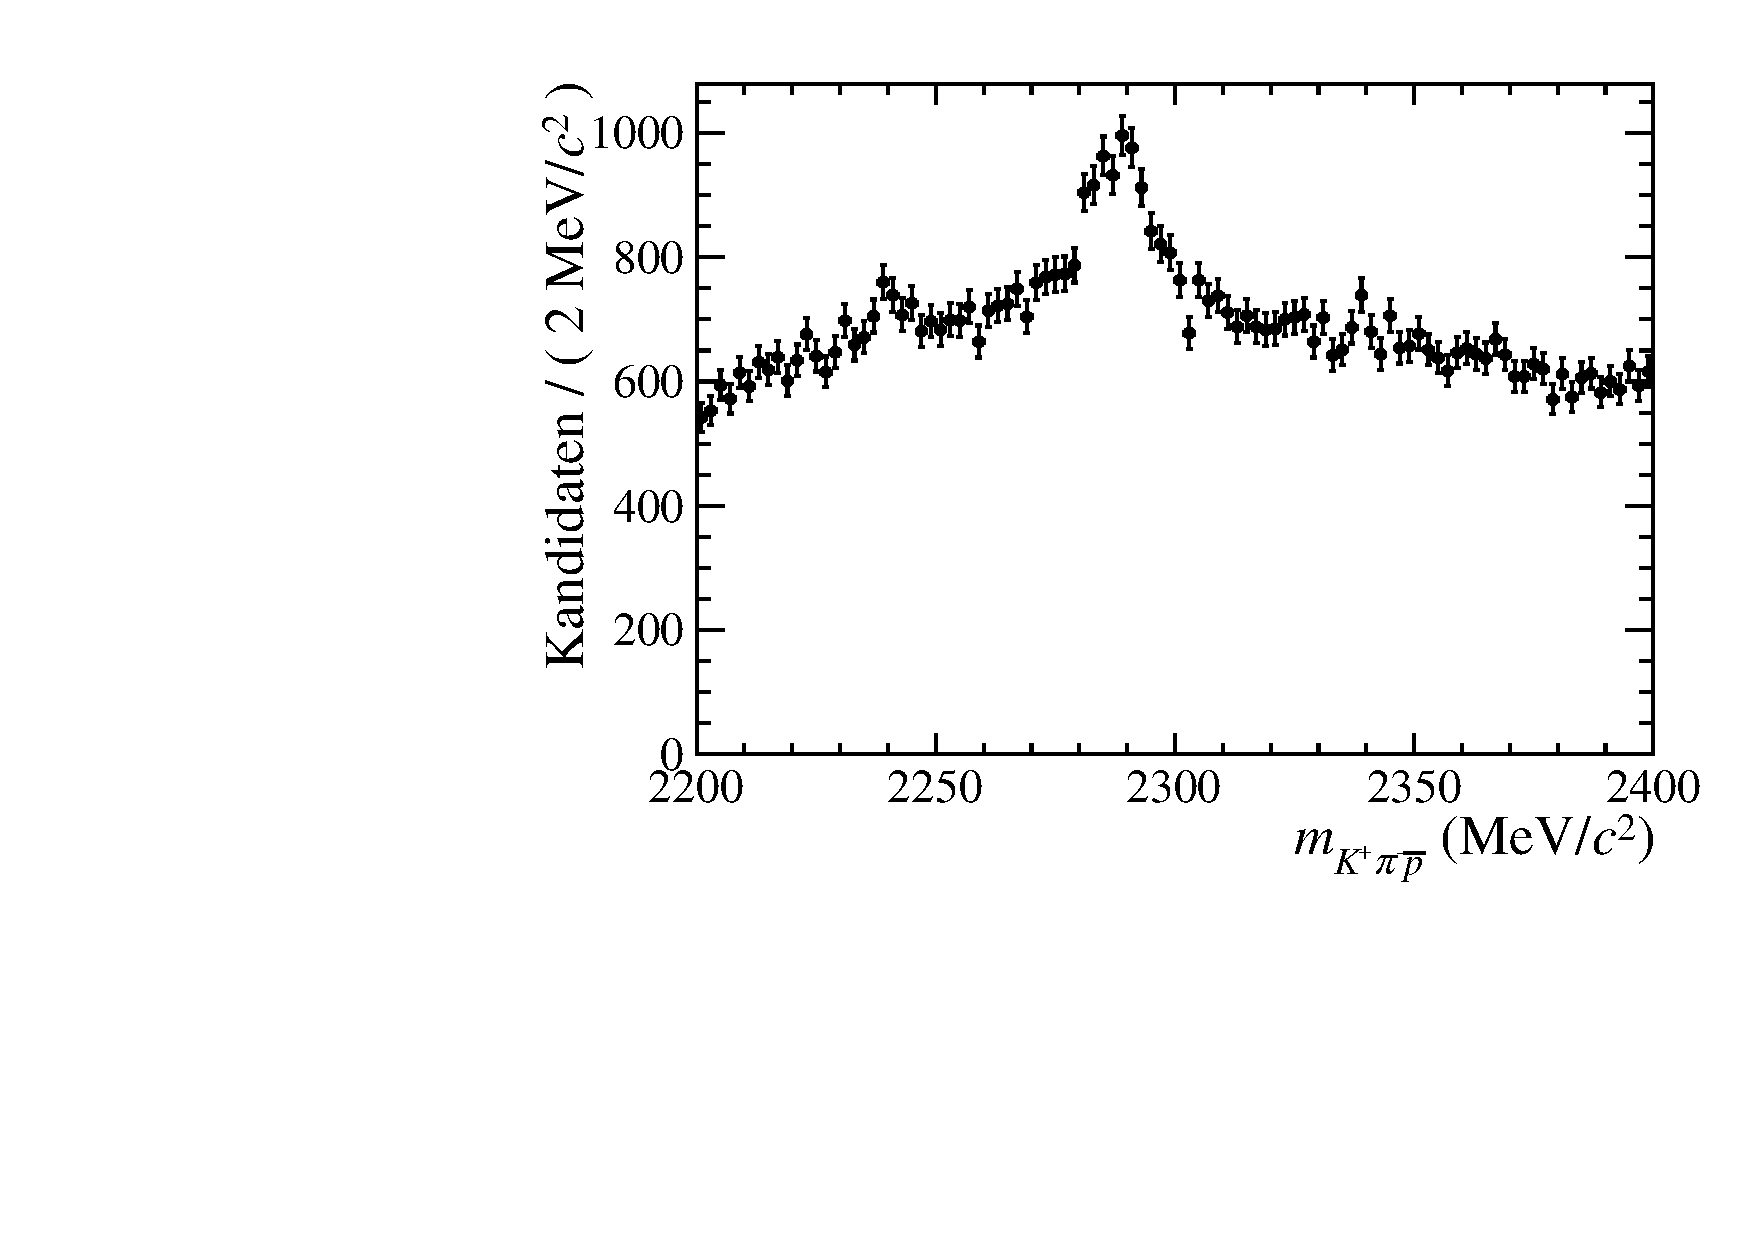
\includegraphics[width=0.45\textwidth]{fig/obsMass_lambda1.pdf}
		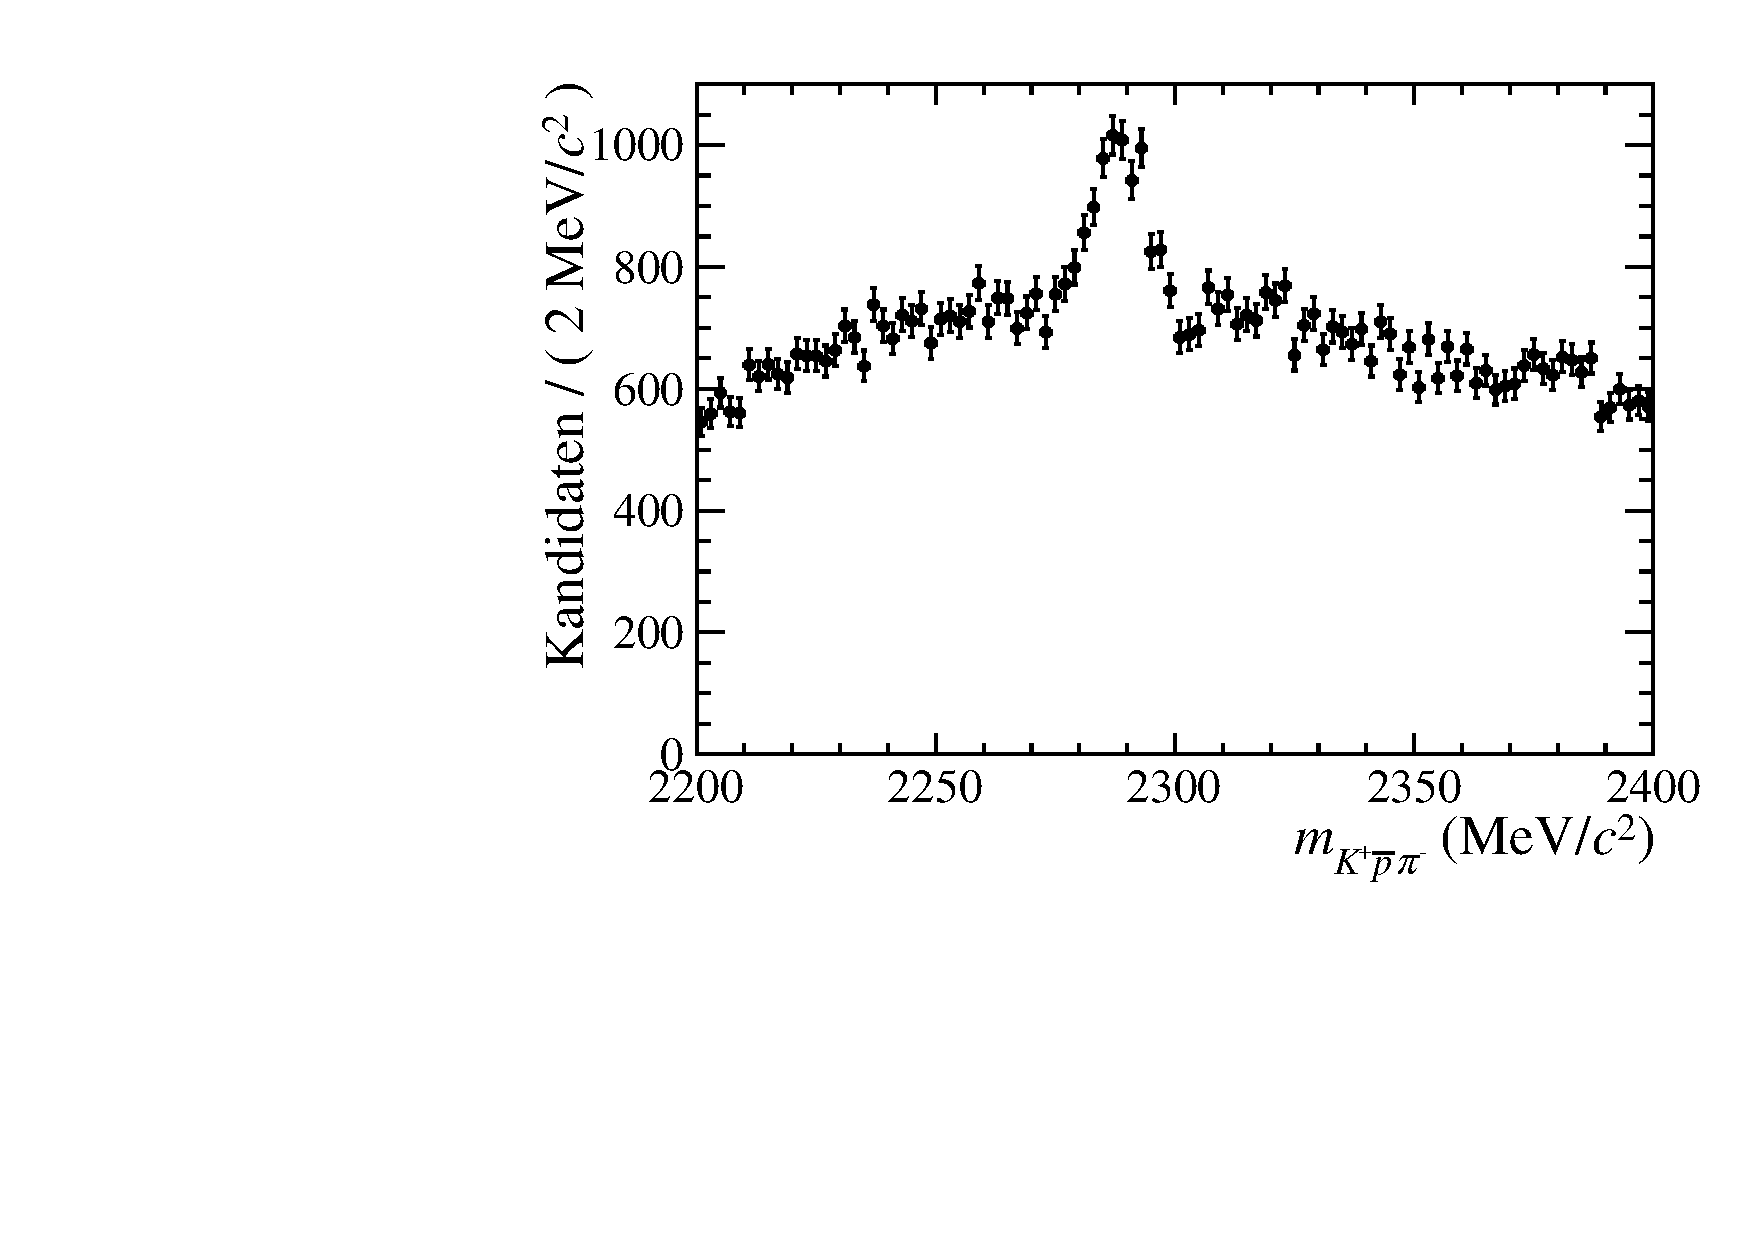
\includegraphics[width=0.45\textwidth]{fig/obsMass_lambda2.pdf}
	\caption{Massenverteilungen der \Kp\pim\pim Kombination nach Anwendung einer Proton Massenhypothese für ein \pim. Die Plots entsprechen den Massenverteilungen für die zwei möglichen Kombinationen.}
	\label{fig:lcveto} 
\end{figure}  
\begin{itemize}
\item Bei dem \Dsm-Veto wird das \Kp mit einem der beiden \pim kombiniert, wobei ein \pim als Kaon fehlidentifiziert wurde. Es wird also nach dem Zerfall $\Dsm\rightarrow\Kp\Km\pim$ gesucht, um einen ähnlichen Endzustand zu bilden wie für das eigentlich gesuchte \Dm-Meson. In Abbildung \ref{fig:dsveto} sind die peakenden Massenverteilungen nach den Kaon Massenhypothesen für die \pim zu sehen. Nach der Kaon Massenhypothese werden Ereignisse mit $\dllkpi>0$ für das jeweilige \pim oder mit einer invarianten Masse innerhalb eines Massenfensters von \SI{30}{MeV\per c^2} um den zentralen Wert der \Dsm-Masse ausgeschlossen. Dabei beschreibt \dllkpi die Wahrscheinlichkeit ob es sich bei einem Teilchen eher um ein Pion oder ein Kaon handelt.
\item Für das \Lc-Veto werden das Kaon und die beiden negativ geladenen Pionen kombiniert, wobei eines der \pim mit einer Proton Massenhypothese versehen wird. Hier soll für das \Lc der Zerfall $\Lc\rightarrow\Km\pip\proton$ gesucht werden. Die peakenden Massenverteilungen nach der Proton Massenhypothese sind in Abbildung \ref{fig:lcveto} dargestellt. Im Folgenden werden nur Ereignisse beachtet, bei denen für das \pim mit der Protonmassenhypothese entweder $\dllppi<0$ gilt oder die Kombination aus \Kp, \pim und \pim mit der Proton Massenhypothese für ein \pim muss außerhalb eines Massenfensters von \SI{30}{Mev\per c^2} um den zentralen Wert der \Lc-Masse sein. Die Größe \dllppi beschreibt hier für ein Teilchen die Wahrscheinlichkeit, ob es sich eher um ein Proton oder Pion handelt.
\end{itemize}
Nach Anwendung aller Schnitte und der beiden Massenvetos ergibt sich eine Signaleffizienz von \SI{67{,}83}{\%} auf Monte-Carlo. Diese Signaleffizienz ist für ein Signal Monte-Carlo für das Jahr \num{2011} berechnet.
 
\section{Verwendetes Fitmodell}

Das Fitmodell für den Kanal $\Bz\rightarrow\Dm\pip$ setzt sich aus einer Signal und einer Untergrund Komponente zusammen. Die \mbox{Wahrscheinlichkeitsdichtefunktion $\mathcal{P}$ (\PDF)} hat daher die folgende Form:
\begin{equation}
N\mathcal{P}(t,\xi,m;\vec{\zeta})=N_\text{Sig}\mathcal{P}_\text{Sig}(t,\xi,m;\vec{\zeta}_\text{Sig})+N_\text{Bkg}\mathcal{P}_\text{Bkg}(t,m;\vec{\zeta}_\text{Bkg}).
\end{equation}
Dabei stellen $m$, $t$ und $\xi$ die beobachteten Observablen (Masse, Zeit und Mischungszustand der \Bz-Mesonen) dar und die $N$ geben die Ereigniszahlen an. Der Mischungszustand ist dabei definiert als $\xi=d\cdot d_f$ mit dem Tag $d$ und dem Zerfallszustand $d_f$. Hat ein \Bz-Meson gemischt ist $\xi=-1$, für ungemischte \Bz-Mesonen gilt $\xi=1$ und bei ungetaggten Ereignissen ist $\xi=0$. Die Signal- (Sig) und Untergrundkomponenten (Bkg) setzen sich weiter als Produkt aus einer \PDF für die Zerfallszeit und für die Masse zusammen
\begin{equation}
\begin{split}
\mathcal{P}_\text{Sig}(t,\xi,m;\vec{\zeta}_\text{Sig})&=\mathcal{P}_\text{Sig,Zeit}(t,\xi;\vec{\zeta}_\text{Sig}^\text{Zeit})\cdot\mathcal{P}_\text{Sig,Masse}(m;\vec{\zeta}_\text{Sig}^\text{Masse})\\
\mathcal{P}_\text{Bkg}(t,m;\vec{\zeta}_\text{Bkg})&=\mathcal{P}_\text{Bkg,Zeit}(t,\xi;\vec{\zeta}_\text{Bkg}^\text{Zeit})\cdot\mathcal{P}_\text{Bkg,Masse}(m;\vec{\zeta}_\text{Bkg}^\text{Masse})
\end{split}
\end{equation}
und werden im Folgenden näher beschrieben.

\subsection{Zerfallszeit Beschreibung}

Die Wahrscheinlichkeitsdichtefunktion zur Beschreibung der Zerfallszeit leitet sich direkt aus den Übergangswahrscheinlichkeiten aus Abschnitt \ref{sec:mixing} ab. Dabei wird eine mögliche \CP-Verletzung in der Mischung vernachlässigt und für beide Masseneigenzustände eine gleiche Zerfallsbreite angenommen. Die vier möglichen Fälle lassen sich schließlich mit der Tagentscheidung $d$ und dem Mischungszustand $\xi$ zusammenfassen zu
\begin{equation}
\mathcal{P}'_\text{Sig,Zeit}(t,\xi;\tau,\dmd,\omega,\Delta\omega,d)\propto e^{-t/\tau}\left[\left(1-d\Delta\omega\right)+\xi\left(1-2\omega\right)\cos\left(\dmd t\right)\right]
\end{equation}
Für die Beschreibung des Untergrundes in der Zeitkomponente wird die \PDF 
\begin{equation}
\mathcal{P}'_\text{Bkg,Zeit}(t,\xi;\tau_\text{Bkg},\omega_\text{Bkg})\propto e^{-t/\tau_\text{Bkg}}\cdot\xi\left(1-2\omega_\text{Bkg}\right)
\end{equation}
genutzt. Der Parameter $\omega_\text{Bkg}$ beschreibt eine tag-Asymmetrie im Untergrund. Neben diesen aus dem Modell des \B-Mesonenzerfalls motivierten Anteilen der Zerfallszeitbeschreibung gibt es allerdings noch zwei weitere  Effekte. \\ 
Zunächst wird die Lebenszeitverteilung durch die Selektion des Zerfalls beeinflusst. Vor allem die HLT Trigger machen Schnitte auf den Stoßparameter des \Bz-Mesons, was kurze Zerfallszeiten beeinflusst. Diese Schnitte sind nötig, um den großen kombinatorischen Untergrund aus Pionen zu unterdrücken, die direkt in den Protonenkollisionen entstehen. Der auftretende Effekt wird dabei mit einer Funktion der Form
\begin{equation}
\epsilon(t)=\arctan\left(t^{a_3}e^{a_1t+a_2}\right)
\end{equation}
beschrieben. Hierbei handelt es sich nicht um ein physikalisch motiviertes Modell, sondern einzig um eine gute Beschreibung des auftretenden Effekts. In Abbildung \ref{fig:akzeptanz} ist das Akzeptanzmodell und sein Einfluss auf die Lebenszeitverteilung dargestellt.
\begin{figure}[tbp]
	\centering
		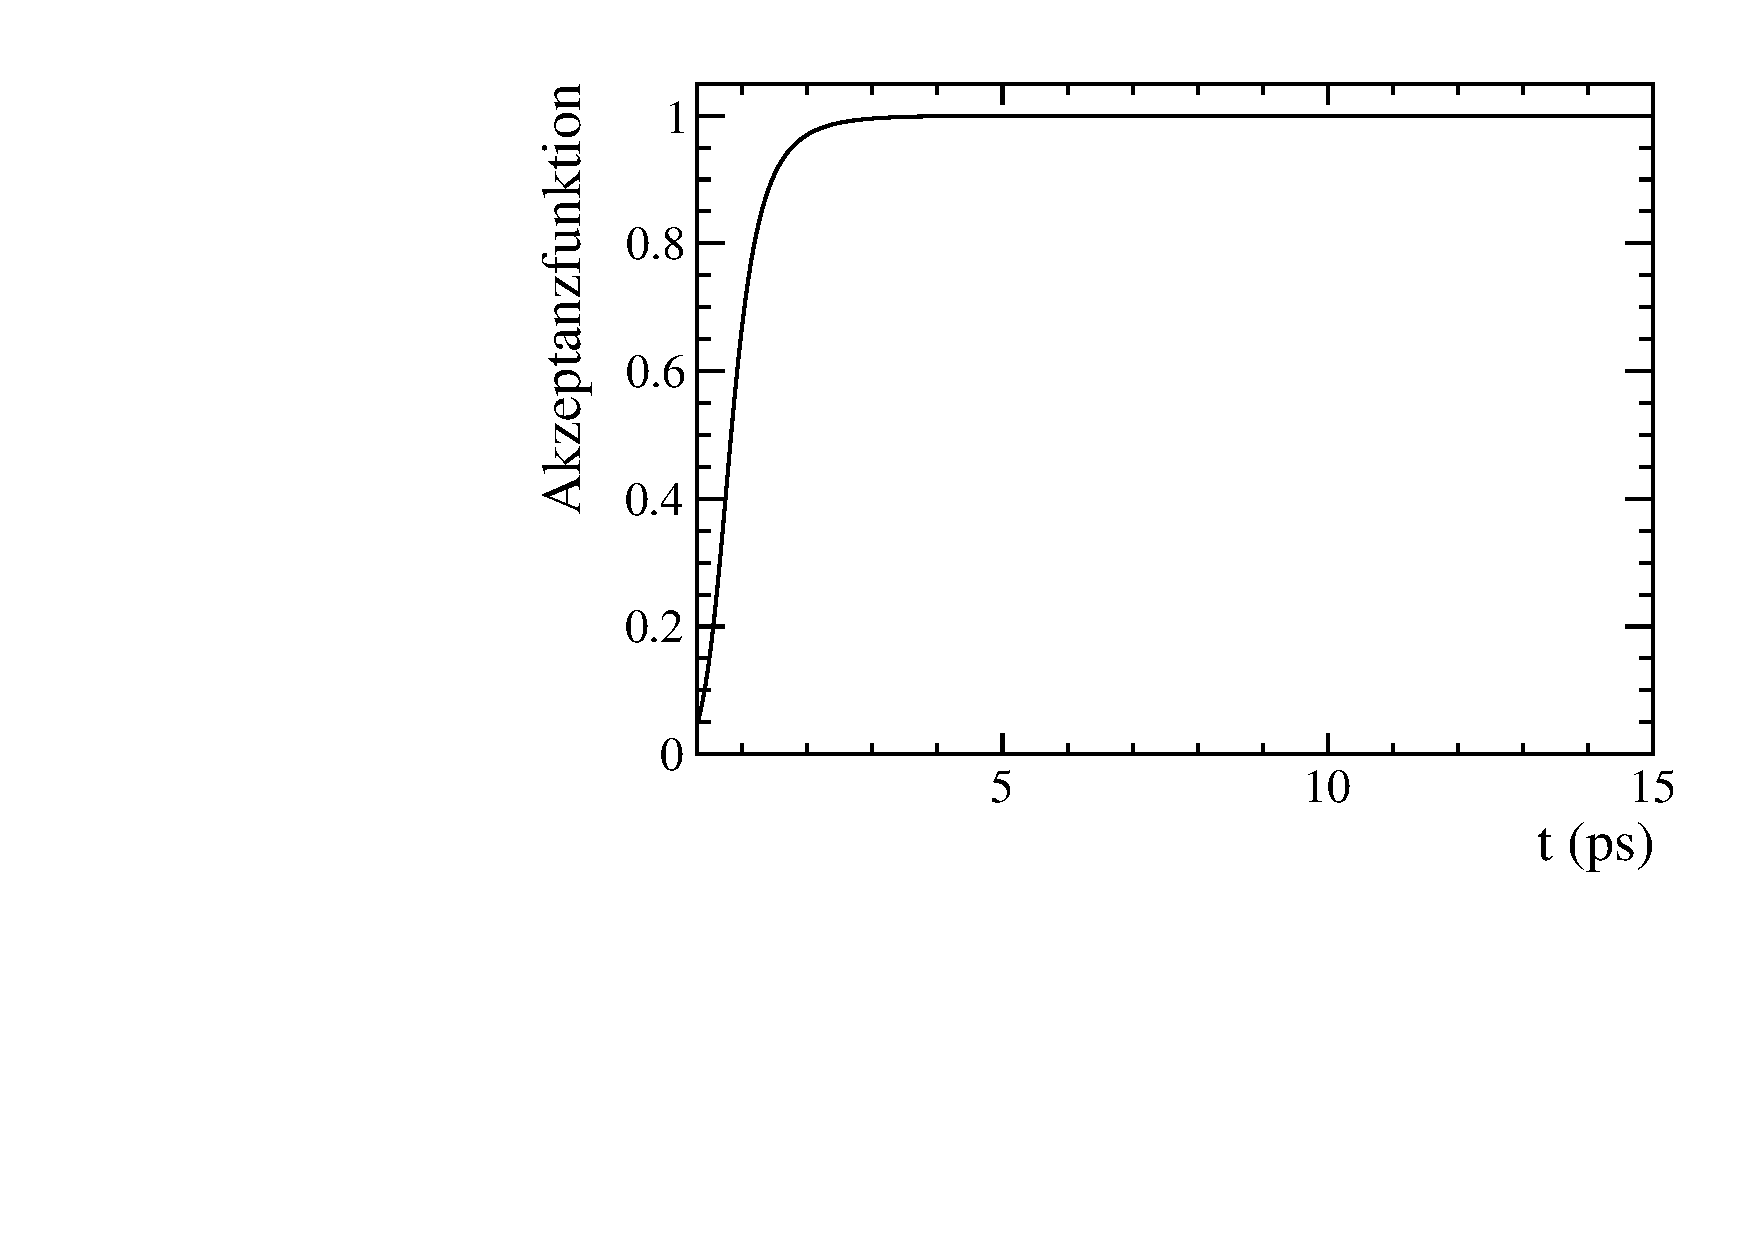
\includegraphics[width=0.45\textwidth]{fig/akzeptanz.pdf}
		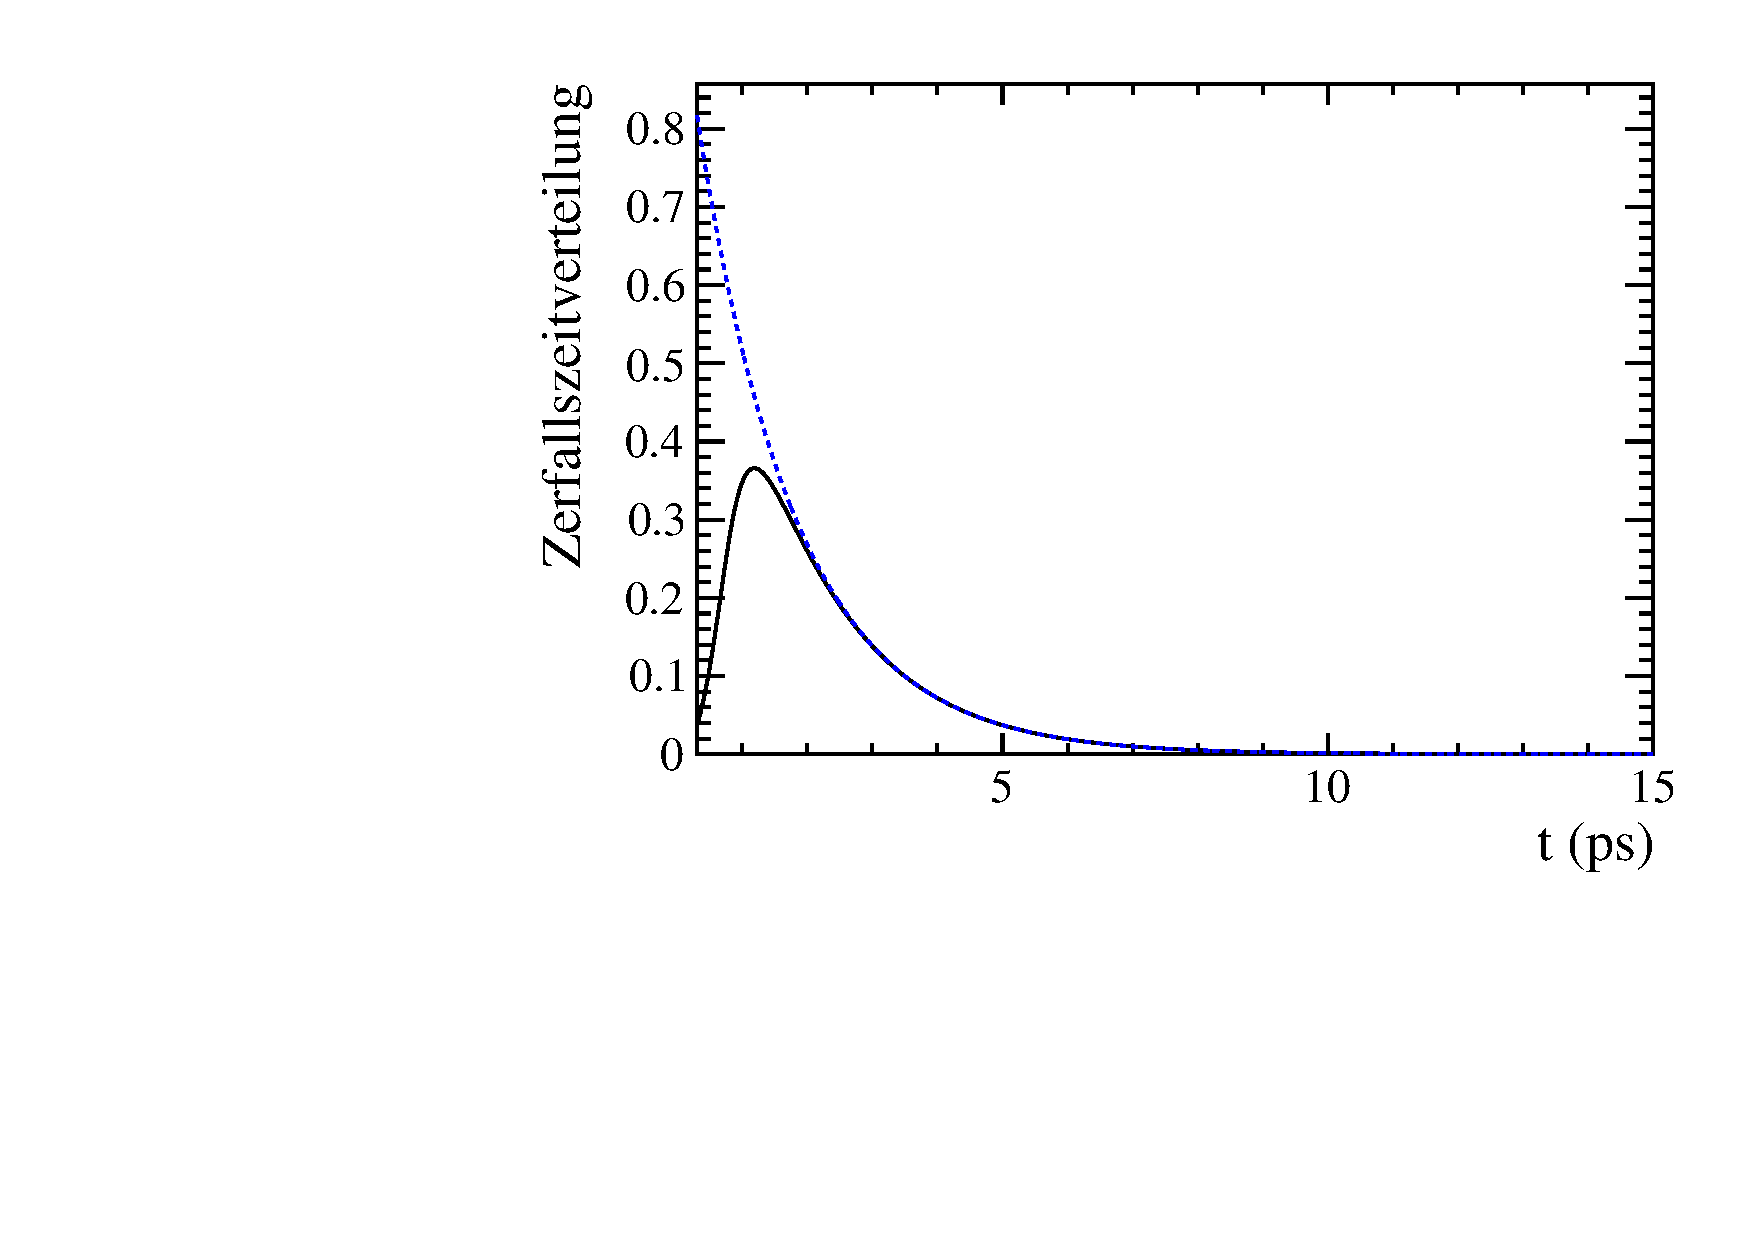
\includegraphics[width=0.45\textwidth]{fig/akzept_expo.pdf}
	\caption{Links die Akzeptanzfunktion die in $\Bz\rightarrow\Dm\pip$ genutzt wird, rechts der Einfluss auf die Zerfallszeitverteilung. In blau gestrichelt ohne und in schwarz mit Akzeptanzeffekt.}
	\label{fig:akzeptanz} 
\end{figure}
Dabei wurde für Signal und Untergrund das gleiche Modell mit  unterschiedlichen Werten für die Parameter $a_1$, $a_2$ und $a_3$ gewählt.\\
Der zweite Effekt, der zu beachten ist, ist die detektorbedingte Zeitauflösung. Hier wurde für Signal und Untergrund das gleiche Modell einer einfachen gaussischen Auflösung 
\begin{equation}
\mathcal{R}(t-t_\text{wahr};s)\propto\frac{1}{s\sqrt{2\pi}}\exp\left(-\frac{\left(t-t_\text{wahr}\right)^2}{2s^2}\right)
\end{equation}
mit einer mittleren Auflösung von $s=\SI{50}{fs}$ verwendet.\\
Insgesamt erhält man so für die Zeitbeschreibung in Signal und Untergrund
\begin{equation}
\begin{split}
\mathcal{P}_\text{Sig,Zeit}(t,\xi;\vec{\zeta}_\text{Sig}^\text{Zeit})&=\epsilon(t)\cdot\mathcal{P}'_\text{Sig,Zeit}(t,\xi;\tau,\dmd,\omega,\Delta\omega,d)\otimes\mathcal{R}(t-t_\text{wahr};s)\\
\mathcal{P}_\text{Bkg,Zeit}(t,\xi;\vec{\zeta}_\text{Bkg}^\text{Zeit})&=\epsilon(t)\cdot\mathcal{P}'_\text{Bkg,Zeit}(t,\xi;\tau_\text{Bkg},\omega_\text{Bkg})\otimes\mathcal{R}(t-t_\text{wahr};s)
\end{split}
\end{equation}

\subsection{Massen Beschreibung}

Als Wahrscheinlichkeitsdichtefunktion für die Masse wurde eine Ipatia Funktion \cite{ipatia}
\begin{multline}
			\mathcal{I}(m;\mu,\sigma,\lambda,\zeta,\beta,a_1,n_1,a_2,n_2) \propto \\
			\begin{cases}
			\left(\left(m - \mu\right)^2 + A_{\lambda}^2(\zeta)\sigma^2\right)^{\frac{1}{2}\lambda - \frac{1}{4}} e^{\beta(m - \mu)} K_{\lambda - \frac{1}{2}}\left(\zeta\sqrt{1 + \left(\frac{m - \mu}{A_\lambda(\zeta)\sigma}\right)^2}\right)	&\, ,  - a_1 < \frac{m - \mu}{\sigma} < a_2 \\
			\frac{G(\mu - a_1 \sigma,\mu,\sigma,\lambda,\zeta,\beta)}{\left(1 - m/(n \frac{G(\mu - a_1\sigma,\mu,\sigma,\lambda,\zeta,\beta)}{G^\prime(\mu - a_1 \sigma,\mu,\sigma,\lambda,\zeta,\beta)} -a_1 \sigma)\right)^{n_1}}	&\, , - a_1 > \frac{m - \mu}{\sigma} \\
			\frac{G(\mu - a_2 \sigma,\mu,\sigma,\lambda,\zeta,\beta)}{\left(1 - m/(n \frac{G(\mu - a_2\sigma,\mu,\sigma,\lambda,\zeta,\beta)}{G^\prime(\mu - a_2 \sigma,\mu,\sigma,\lambda,\zeta,\beta)} -a_2 \sigma)\right)^{n_2}}	&,\quad a_2 < \frac{m - \mu}{\sigma} \\
			\end{cases}
			\label{eq:ipatia}
		\end{multline}
mit 
\begin{equation}
\begin{split}
&G(m,\mu,\sigma,\lambda,\zeta,\beta,a,n)\propto\\
&\left(\left(m-\mu\right)^2+A_\lambda^2(\zeta)\sigma^2\right)^{\frac{1}{2}\lambda-\frac{1}{4}}e^{\beta\left(m-\mu\right)}K_{\lambda-\frac{1}{2}}\left(\zeta\sqrt{1+\left(\frac{m-\mu}{A_\lambda(\zeta)\sigma}\right)^2}\right)
\end{split}
\end{equation}
benutzt. Dabei beschreibt $\mu$ den Mittelwert, $\sigma$ die Standardabweichung und die Parameter $a_i$ und $n_i$ mögliche exponentielle Ränder der Verteilung. Diese können entstehen, wenn beispielsweise durch Wechselwirkungen mit dem Magnetfeld Photonen emittiert werden (Verschiebung zu niedrigen Massen) oder Detektoreffekte (Verschiebung zu hohen Massen). Für den Untergrund wird eine Exponentialfunktion der Form
\begin{equation}
\Epsilon(m;M)\propto e^{\frac{m}{M}}
\end{equation}
gewählt um den kombinatorischen Untergrund zu beschreiben. Es ergibt sich also
\begin{equation}
\begin{split}
\mathcal{P}_\text{Sig,Masse}(m;\vec{\zeta}_\text{Sig}^\text{Masse})&=\mathcal{I}(m,\mu,\sigma,\lambda,\zeta,\beta,\alpha,n)\\
\mathcal{P}_\text{Bkg,Masse}(m;\vec{\zeta}_\text{Bkg}^\text{Masse})&=\Epsilon(m;M)\propto e^{\frac{m}{M}}.
\end{split}
\end{equation}
